\documentclass[paper=a4, fontsize=11pt]{scrartcl}
\usepackage[T1]{fontenc}
\usepackage{fourier}
\usepackage[english]{babel}
\usepackage[protrusion=true,expansion=true]{microtype}	
\usepackage{amsmath,amsfonts,amsthm} % Math packages
\usepackage[pdftex]{graphicx}	
\usepackage{url}
\usepackage[style=authoryear-icomp,sorting=anyt]{biblatex}
\addbibresource{sample.bib}
\usepackage{float}
\usepackage{sectsty}
\allsectionsfont{\centering \normalfont\scshape}
\usepackage{fancyhdr}
\pagestyle{fancyplain}
\fancyhead{}										% No page header
\fancyfoot[L]{}											% Empty 
\fancyfoot[C]{}											% Empty
\fancyfoot[R]{\thepage}									% Pagenumbering
\renewcommand{\headrulewidth}{0pt}			% Remove header underlines
\renewcommand{\footrulewidth}{0pt}				% Remove footer underlines
\setlength{\headheight}{13.6pt}


%%% Equation and float numbering
\numberwithin{equation}{section}		% Equationnumbering: section.eq#
\numberwithin{figure}{section}			% Figurenumbering: section.fig#
\numberwithin{table}{section}				% Tablenumbering: section.tab#


%%% Maketitle metadata
\newcommand{\horrule}[1]{\rule{\linewidth}{#1}} 	% Horizontal rule

\title{
		%\vspace{-1in} 	
		\usefont{OT1}{bch}{b}{n}
		\normalfont \normalsize \textsc{Technical University of Darmstadt $ \bullet$ 2018} \\ [25pt]
		\horrule{0.5pt} \\[0.4cm]
		\huge Project: Packet Inspection for Malware Detection \\
        \small (new version) \\
		\horrule{2pt} \\[0.5cm]
}
\author{
		\normalfont 								\normalsize
        Nurefsan SERTBAS\\[-3pt]		\normalsize
        \today
}
\date{}


%----------------------------------------------------------------------------------------
\begin{document}
\maketitle % Insert title
\section{Introduction}
In this section, we extend our implementation considering following cases:


\begin{itemize}
    \item Unlike the previous version which only considers the TCP packets, current implementation considers both TCP and UDP packets.
    \item We did not considered the non-printable characters in packet payload. However, we fix that issue in current version.
\end{itemize}



\section{Implementation Details}
You can compile and run the program with the same commands as in previous version. 

To test our new version, we have sent two packets (one for TCP and one for UDP) to the target host. We use the code given in following figure.

\begin{figure}[H]
\centering
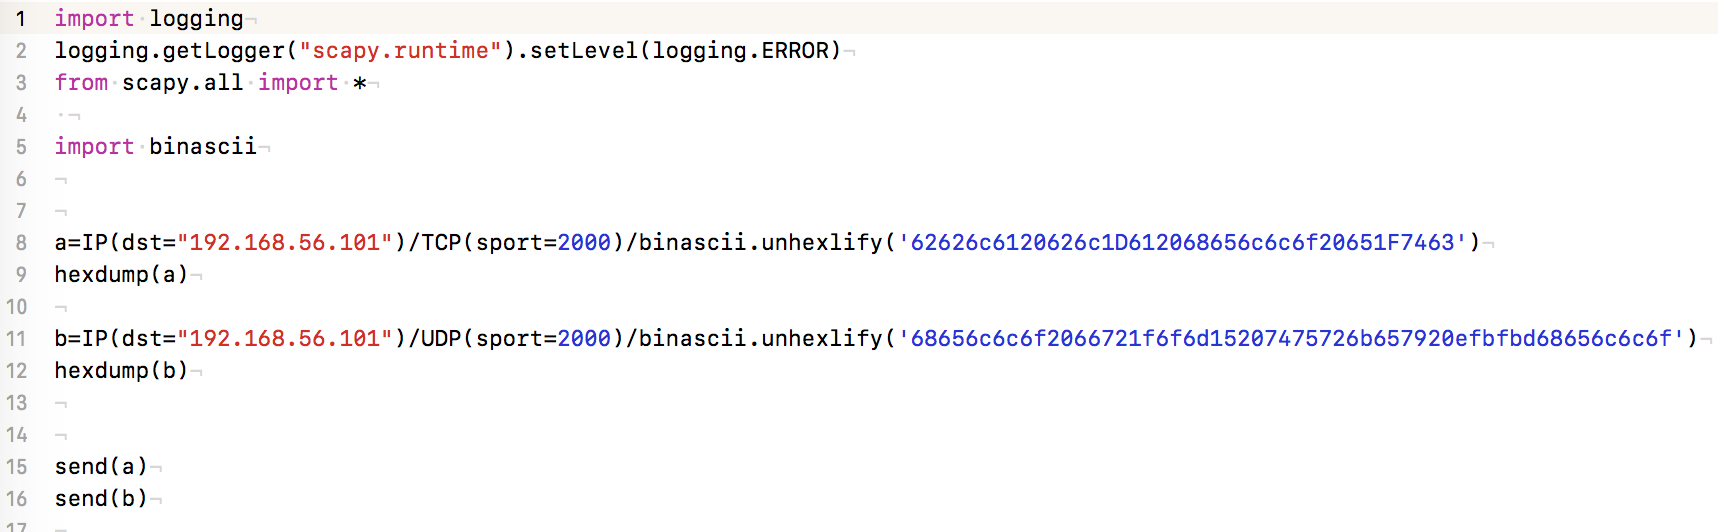
\includegraphics[width=\textwidth]{img2/traffic.png}
\caption{Content of the traffic file for testing}
\end{figure}

The non-printable character codes are obtained from \cite{r5} and can be checked via \url{http://www.unit-conversion.info/texttools/hexadecimal/}. We start to listen incoming TCP and UDP packets at target host. Then, we sent the traffic whose content is given in Figure \ref{traffic}.

\begin{figure}[H]
\centering
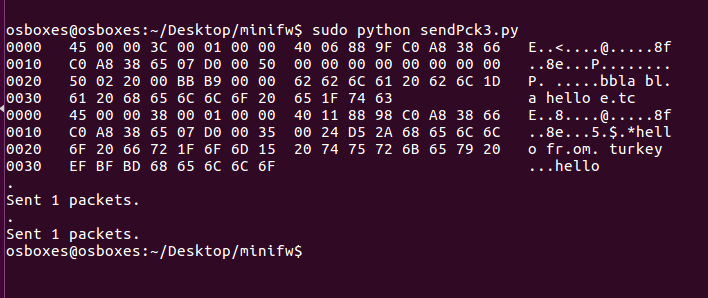
\includegraphics[width=\textwidth]{img2/utraf.png}
\caption{Sent packets} \label{traffic}
\end{figure}

After that, the captured packets and corresponding processing details are given in Figure \ref{res}.
\begin{figure}[H]
\centering
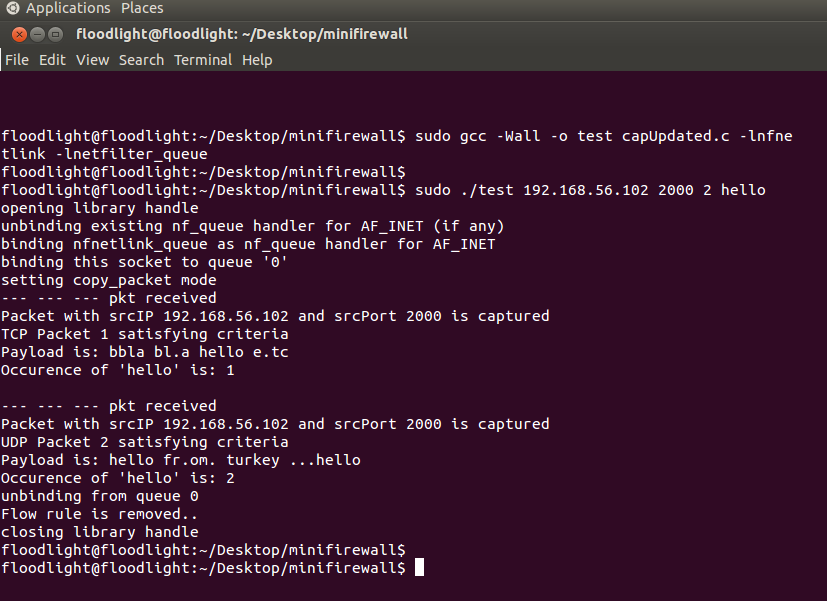
\includegraphics[width=\textwidth]{img2/ures.png}
\caption{Results of the program (capUpdated.c)}\label{res}
\end{figure}

The code successfully captures the desired sub-string (hello in the example) and counts its occurrences. Finally, the content of the produced output.txt file is given in following figure.

\begin{figure}[H]
\centering
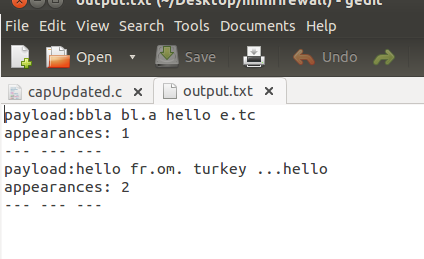
\includegraphics[width=\textwidth]{img2/uout.png}
\caption{Content of the output.txt}
\end{figure}

Note that, non-printable characters are represented via '.' in both command line and the output.txt file.


\section*{Additional Notes}
\begin{itemize}
\item Project code and documentation can be accessed on \url{https://github.com/sertbasn1/minifirewall.git}.
\item In the implementation we only listen eth1 with following implicit rule '"sudo iptables -A INPUT -i eth1 -j NFQUEUE --queue-num 0"'. There is no special reason for selecting eth1 interface.
\item For the sake of simplicity, we implicitly set dest port as 2000 and dest ip as 192.168.56.101 in sendPckt.py
\end{itemize}

\printbibliography
\end{document}